\chapter{Problem Statement and Solution Overview}\label{chapter:solution}
In this chapter, the formal setting of our case study will be given. We will also demonstrate some key issues and main challenges in this problem. Then we will deliver our pipeline and solution overview for ontology-based visual analytics for text analysis.

\section{Problem Statement}
This project is going to solve the problem of integrating and visualising useful information from a large number of web pages. The biggest challenge of the project is acquiring requisite data from various HTML web pages by using semantics web technologies and transferring the data to the corresponding ontologies for the visualisation. About only a few decades ago, this was considered as an impossible task. Nowadays, with the help of ontologies, automated text processing becomes conceivable\cite{krallinger2012link}.

As we stated above, because of the development of information technology and cyberspace, data is growing exponentially on the internet. A piece of useful information is often mixed with irrelevant data or shown on different web pages redundantly. Meanwhile, the information is presented in a great diversity of ways and thus makes it more difficult for humans to handle and integrate\cite{anantharangachar2013InfoExtraction}. In this chapter, we will firstly using seminar announcement pages in University of Oxford as the example to state the complexity and difficulty of this problem.

First of all, for the purpose of getting all the seminar announcements, it is necessary to crawl all the web pages in the entire website of University of Oxford. However, our research object is information that very sensitive to time, such as seminar announcements. Every hour and every day, numerous seminar announcements webpages are created, updated or deleted. Seizing these changes efficiently and accurately is a big challenge for our system. 

\begin{figure}[htb!]
	\centering
	\includegraphics[page=2,width=\textwidth]{images/picture.pdf}
	\caption{Examples: Target Page and Non-Target Page}\label{fig:emp:target_vs_non}
\end{figure}

\begin{figure}[htbp!]
	\centering
	\includegraphics[page=3,width=0.93\textwidth]{images/picture.pdf}
	\caption{Examples: Various Presentation of Seminar Announcement}\label{fig:emp:various_present}
\end{figure}

Next, how to distinguish between our target webpage(i.e. seminar announcement page) and the large amount of the webpages crawled by the system is still a complex problem. For instance, the two webpage screenshots in Figure \ref{fig:emp:target_vs_non} both contain indicators\footnote{e.g. `\textbf{Date:}',`\textbf{Time:}',`\textbf{When:}'} and entities\footnote{e.g. `Fri, 24 Jul 2015',`10:00',`24th June 2015'} about date and time, name and location information. They also have a great similarity of page layout between each other. Meanwhile, there are many seminar announcements pages with totally different page layouts (such as Figure \ref{fig:emp:various_present}) too. It is extremely hard for a machine to tell the difference and further decide whether they are seminar announcement pages. A machine could make a decision in next to no time but with low accuracy. However, it is easy for a human to judge as long as he understands English, and the result will be much more accurate than a machine.

Despite of this, there are other problems. One of the most troublesome challenges among them is data extraction from natural language and processing the ontology integration automatically\cite{maedche2003bootstrapping}. Although we have confirmed a web page contains seminar information, extracting those information is still not easy. For example, consider these three seminar announcement web pages from different departments (see Figure \ref{fig:emp:various_present}). 

The first screenshot comes from the Mathematical Institute\footnote{ \url{https://www.maths.ox.ac.uk/node/14127} at 01:00, 27th Jul 2015 }. We could see that related information such as `31 August 2015 09:00', `L3' and `Derived structures in geometry and representation theory' are in different grids. But there is no distinct indicator word (such as `Date', `Time' and `Location') to indicates. The second screenshot comes from the the Cyber Security Centre in Department of Computer Science\footnote{ \url{http://www.cs.ox.ac.uk/seminars/1439.html} at 01:00, 27th Jul 2015 }. Information such as time and location are listed corresponding to each indicator. Speaker and title are stated separately in the header. Unlike the previous two, the third screenshot (department of physics)\footnote{ \url{http://www2.physics.ox.ac.uk/research/seminars} at 01:00, 27th Jul 2015 } contains many seminar announcement information and listed in a table. It can be seen that webpages are very diverse from content to layout. Although we are able to capture these information fast manually, it is extremely difficult for a machine to extract the implied structured information based on only one or a few general rules.

Nevertheless, these are the main parts we captured from the entire webpage. Usually, they are wrapped in a lot of irrelevant information. Thus, making use of the extraction on the core parts is also a problem. Furthermore, there is no existing data set. We need to get the entire data set, both training data and test data for the experiments, manually by ourselves.

\section{OXSEM Dataset}
In the domain of seminar announcement webpages, there is no existing labelled dataset. In order to test and conduct experiment on our solution, after labelling and re-check more than 1500 webpages in oxford websites manually, we create a seminar announcement webpages dataset -- \textbf{OXSEM}. It includes 1300 data records:

\begin{table}[htb]
\small
\centering
\caption{Data Distribution of OXSEM Dataset}
\label{tab:dataset}
\begin{tabular}{@{}lll|l@{}}
\toprule
Single Target Page & Multiple Targets Page & Non-Target Page & Total \\ \midrule
400                & 200                  & 700             & 1300    \\ \bottomrule
\end{tabular}
\end{table}
Each data entity contains its original HTTP response and its label(Single Target Page/Multiple Targets Page/Non-Target Page), and this dataset covered dozens of departments or colleges's website in University of Oxford.

\section{Solution Architecture Overview}
It can be seen that the problem stated above needs a systematic solution. Our solution gives a multi-agent system which makes it possible to solve this problem by using a pipeline combined with machine learning and visual analytics.

In general, the system we provide here, named \textbf{SAE} has a clear architecture(see Figure \ref{fig:sys:arch}), which consists of four agents: Crawlers(Retriever and Checker), Filter, Extractor and Presenter. Meanwhile, a well-designed Web User Interface is used to control these agents. A relational database with two tables is responsible for storing the URL addresses and the target information.

\begin{figure}[htb]
	\centering
	\includegraphics[page=1,width=0.9\textwidth]{images/diagrams.pdf}
	\caption{Solution Architecture}\label{fig:sys:arch}
\end{figure}

\begin{itemize}
  \item \textbf{Interaction Layer}\\
  This layer is responsible for communication and interaction with the end users.
  \item \textbf{Knowledge Layer}\\
  This layer contains knowledge for classification and extraction in the target area context. Specifically, the knowledge exists in the form of ontology.
  \item \textbf{Processing Layer}\\
  This is the automatic processing layer, which is responsible for the entire processing procedure including data collecting, webpage classification, and information extraction.
  \item \textbf{Store Layer}\\
  This layer is used to store related information of URLs and entities in order to achieve data persistence.
\end{itemize}

\noindent The four agents are implemented in Python, and are dealing with the four key phases in this problem respectively.

\subsection{Crawler}
As the webpages on the internet are created and updated frequently, the data set in the real world is always changing. Therefore, we implemented a high-efficiency and highly customisable spider program to fulfil the need of acquiring web data with higher degree of liberalisation. Crawlers are not intelligent. They are not able to decide whether or not they need to crawl further and deeper based on the content of the current page. This is because the target page might be at the deeper reaches of the webpages that seems to be irrelevant.

Crawler is an agent which uses blind commitment strategy. The agent who uses this strategy will maintain its goal(intention) and try to fulfil requirements of reaching the goal until it believes the goal has been successfully achieved. It is also sometimes referred to as fanatical commitment \cite{Wooldridge:2009:IMS:1695886}.

Broad crawler is very suitable to solve this problem. Nevertheless, we need to make it become highly customisable as we have different settings for different topics. For example, we need another setting to solve the university programs question we mentioned before. On account of the seminar announcement type of task particularly, we specifically designed two crawlers.

The two crawlers are considered as one \textbf{Retriever} and one \textbf{Checker}.

The \textbf{Retriever} crawls every webpage in the domain of the University of Oxford (ox.ac.uk). It has a long running time, which makes it time consuming. Fortunately, it does not have to run in short cycles, once a week is enough. As \textbf{Retriever} is focusing on the structure or layout changes of the website, it is only required to run when the structure or layout of a website has critical updates.

The \textbf{Checker} revisits the URLs that has been marked as the target pages in the database. It only crawls afresh the target pages which content has been updated. For example, when the location information of a seminar is changed, the announcement webpage will be modified and updated. When this happens, the \textbf{Checker} will capture this and put this webpage in the pipeline again. The \textbf{Checker} has much shorter running time because of its purpose and features. Thus, it could run more frequently, such as once a day.

\subsection{Filter}
We need to screen out those seminar announcement pages from the webpages obtained by the crawlers. We implemented an automatic \textbf{Filter} to take charge of this job, with approximate 90\% correctness. This \textbf{Filter} extracts features by using ontology in the target area provided by the expert. We use decision tree as the classifier and with the	addition of human visual analytics. This makes this automatic \textbf{Filter} be more accurate and more suitable for the job. \textbf{Filter} will act as a daemon process and keeps running all the time. Hence, its socket will always be running as well to receive command messages from other agents or human. Due to its complexity, we will introduce the design and implementation of \textbf{Filter} in details in Chapter \ref{chapter:clf}.

\subsection{Extractor}
The target pages screened out by the \textbf{Filter} implied all the structured data we need. We implemented a semi-automatic \textbf{Extractor} for the purpose of extracting structured data from the unstructured text files. With the assistance of visual analytics, users are able to create extraction ontology or directly make use of the existed ontology to extract target information. It makes the process of extracting data from various different webpage structures become easy and feasible. \textbf{Extractor} will also act as a daemon process and keeps running all the time. Due to its complexity, we will present the design and implementation of \textbf{Extractor} specifically in Chapter \ref{chapter:ie}.

\subsection{Presenter}
The system requires different visualisation models for different study cases in order to present the information fetched from the \textbf{Extractor}. For instance, with regard to seminar announcements, we need to provide a calendar view for the end users to get a intuitional impression. This makes the entire system complete and applicable. 

\subsection{Database and File Storage}
These components are used to store the information about the HTTP response and the extracted seminar announcements. From the introductions above, we could easily find that both \textbf{Filter} and \textbf{Extractor} need the original http response downloaded by the crawlers. With the purpose of preventing duplicate downloads, we use file system to store these original http response. For dynamic data, we designed a database shown in Figure \ref{fig:sys:db}.

\begin{figure}[htb]
	\centering
	\includegraphics[page=9,width=0.8\textwidth]{images/diagrams.pdf}
	\caption{Database Schema Design}\label{fig:sys:db}
\end{figure}
\begin{itemize}
	\item \texttt{url\_lib} is used to store the related information of webpages crawled by the crawlers, including \texttt{url},\texttt{title},\texttt{content\_type}. Additionally, \texttt{is\_target} is used to mark the classification decision of the target webpage, while \texttt{content\_hash} will record the hash value of the original response so that it is able to determine whether the content has been updated when crawling again later. \texttt{layout\_hash} will record the hash value of the webpage's layout\footnote{we will introduce the definition of the layout in Section \ref{defn:layout} in page \pageref{defn:layout} } in order to determine whether the webpage has the same layout later. And\texttt{extractor} will record the extractor corresponding to this url.
	\item Another table is used to store the extracted entity and attributes. In this case, \texttt{sem\_info} is used to store the attributes of extracted seminar information. In other cases, we need to change the structure of this table.
\end{itemize}

\subsection{Web Interface}
In order to make artificiality get involved in the entire process with the assistance of visual analytics. It helps with improving the accuracy of webpage classification and information extraction. Particularly, we designed a web interface to interact with the agents such as \textbf{Filter} and \textbf{Extractor}. It was implemented by using the current popular Python Web framework: Django\footnote{\url{https://www.djangoproject.com}
}.

Here, we only give some overview screenshots. The specific operations of the web interface will be explained in the following chapter.

\begin{figure}[htb]
	\centering
	\includegraphics[page=4,width=0.8\textwidth]{images/picture.pdf}
	\caption{Web Interface Screenshots}\label{fig:sys:webui}
\end{figure}


\section{Solution Pipeline}
The system contains the entire procedure including data collection, classification, extraction and presentation. It also combines machine learning with visual analytics under human-computer interaction. On the premise of high efficiency, it greatly improves the accuracy and solved these kind of problem well. Next, we will explain the pipeline of the solution in detail based on the above system architecture. Specifically, we are going to take the view of webpage data to expound the pipeline with the help of the combination of pipeline (Figure \ref{fig:sys:pip}) and data flow (Figure \ref{fig:sys:data_flow}).

From Figure \ref{fig:sys:pip}, it could be seen that the whole pipeline is consist of four stages below:
\begin{figure}[htb]
	\centering
	\includegraphics[page=2,width=\textwidth]{images/diagrams.pdf}
	\caption{Solution Pipeline}\label{fig:sys:pip}
\end{figure}

\subsection{Stage1: Crawl Webpages}
Firstly, like in \ref{fig:sys:data_flow}, crawlers will crawl particular webpages in the assigned domain according to the start URLs and some constraints given by human experts. These constraints for our mission is shown in Table \ref{tab:crawler_constraints}.
\begin{figure}[htb!]
	\centering
	\includegraphics[page=3,width=\textwidth]{images/diagrams.pdf}
	\caption{Pipeline Data Flow}\label{fig:sys:data_flow}
\end{figure}

\begin{figure}[htb!]
	\centering
	\includegraphics[page=5,width=0.9\textwidth]{images/diagrams.pdf}
	\caption{Flow Chart for Crawler}\label{fig:fc:crawler}
\end{figure}

\begin{table}[htb!]
\small
\centering
\caption{Crawler Constraints}
\label{tab:crawler_constraints}
\resizebox{\textwidth}{!}{%
\begin{tabular}{@{}p{0.3\textwidth}p{0.3\textwidth}p{0.4\textwidth}@{}}
\toprule
\textbf{Constraint} & \textbf{Description} & \textbf{Setting in  This Case} \\ \midrule
\texttt{allow\_content\_type}	& Allowed \texttt{content-type} in the http response header                 & \texttt{["text/html"]}\\ \midrule
\texttt{allow\_domains}	& domains which allow crawlers to scan & \texttt{["ox.ac.uk"]}\\ \midrule
\texttt{deny\_domains}	& domains which deny crawlers to scan & \texttt{["webauth.ox.ac.uk", "weblearn.ox.ac.uk"]}\\ \midrule
\texttt{deny\_extensions}	& file extensions that the crawlers will not follow & \texttt{[
    "pdf", "doc", "docx", "xls", "xlsx", "ppt", "pptx", "png", "jpg", "gif", "ps", "tex", "bib", "zip",
    "tar", "gz", "tgz", "java", "cpp", "c", "scala", "msi", "exe", "sh", "com", "bin", "mp4", "avi"]}\\ \midrule
\texttt{deny\_deny\_regxs}	& the urls will be ignored if these regular expressions matched & N/A \\ \midrule
\texttt{deny\_max\_url\_length}	& maximum length of the allowed url & \texttt{512}\\ \midrule
\texttt{deny\_download\_time\_out} & time(in seconds) that the crawler will retry the page downloading & \texttt{2}\\ \midrule
\texttt{deny\_depth\_limit}	& search depth of the crawler & \texttt{4}\\
\bottomrule   
\end{tabular}
}
\end{table}

When the \textbf{Retriever} use these constraints to get an http response, check the \texttt{url\_lib}. If this URL has already been in the database, calculate the hash value of the response content and compare the calculation result with the \texttt{content\_hash} in the \texttt{url\_lib}, so that it could determine whether the webpage has updated. Once it discovers that the webpage has updated, in order to maintain the consistency of the system and the content, \textbf{Retriever} will delete all the record related to this URL in the \texttt{url\_lib} and \texttt{sem\_info}. Meanwhile, this URL is regarded as a URL which never exists in the \texttt{url\_lib} and forms a new record. Then, the response html of this URL will continue be extracted, and the related information of this record will be stored in the \texttt{url\_lib}. Furthermore, the corresponding content will be sent to \textbf{Filter} by the communication protocol defined by us.

In addition, we have a similar agent called \textbf{Checker}, which is responsible for checking whether the webpages marked as `target' in the \texttt{url\_lib} have updated. The only difference between \textbf{Checker} and \textbf{Retriever} is that the \texttt{start\_urls} for \textbf{Checker} are only the webpage records that has been marked as `target' in the \texttt{url\_lib}. Besides, the \textbf{Checker} will not go deeper to get further links.


\subsection{Stage2: Filter Webpages}
When Filter receives the message sent from crawlers (because of the features of crawlers we stated above, these URLs are considered as brand new links by the system), it will first use a built-in Feature Extractor to extract the webpage into a feature vector. Then, it uses a pre-trained decision tree classifier to classify this feature vector. Meanwhile, our \textbf{Filter} will give out a confidence value corresponding to the classification result. When the confidence value is higher than a pre-defined threshold, the system will make the decision automatically, and then send it to the \textbf{Extractor} through communication protocol for further processing if it is a target page. Otherwise, the URL will be put into a judge list and handled manually in order to make the accuracy of the classification result as high as possible. On the other hand, the human interaction here will also make the automatic filtering system become stronger through the active learning process.

The detailed procedure of Feature Extract and Classification is complicated. Thus, we will deliver specific explanations to them separately in Chapter \ref{chapter:clf}.

\subsection{Stage3: Generate/Retrieve Rules and Extract Information}
When the \textbf{Extractor} receives the candidate pages selected by the \textbf{Filter}, it will put the pages into a list. The \textbf{Extractor} will choose a suitable extractor instance to extract required information based on the existing records in the database. If there is no such proper extractor instance, user can create an extractor instance which fits this webpage with the help of visualisation and ontology. Then the system will extract out a tuple that contains attributes of seminar announcement information according to the extractor instance. Additionally, user is able to fast judge whether a candidate page in the \textbf{Extractor}'s list has been marked wrong with the assistance of visualisation. Those pages that were decided incorrect will be send back to the \textbf{Filter} to amend its classifiers. 

\subsection{Stage4: Visualisation}
The last step is presenting our system result in an appropriate way. For seminar announcements, we choose to use the calendar view shown in Figure \ref{fig:sys:pre}. More presentation modes will be introduced in later chapters.

\begin{figure}[htb!]
	\centering
	\includegraphics[page=12,width=\textwidth]{images/picture.pdf}
	\caption{Calendar View}\label{fig:sys:pre}
\end{figure}

\subsection{Communication Protocol}
In this multi-agent system, the communications between these agents are quite large and frequent. Therefore, we designed a set of communication protocol and let the agents communicate through the combination of asynchronous socket and file system. This makes the pipeline persistent and efficient.

First of all, \textbf{Filter} and \textbf{Extractor} both have a \texttt{inbox} folder in the file system. The original http response will move among these agents' inbox. Together with the following commands\footnote{in order to serialise the command, it uses \texttt{pickles} package to dump and load these commands} send and receive through the socket of agents, which makes the consistency and efficiency of the whole system. We list the protocols for the sockets of \textbf{Filter} and \textbf{Extractor} correspondingly in the two tables below.
\begin{table}[htb]
\small
\centering
\caption{Socket Protocols for Filter}
\resizebox{\textwidth}{!}{%
\begin{tabular}{@{}p{0.20\textwidth}p{0.26\textwidth}p{0.22\textwidth}p{0.32\textwidth}@{}}
\toprule
  \textbf{Command}   
& \textbf{Parameters}
& \textbf{Response}
& \textbf{Description} \\ 
	\midrule \texttt{new}
	& \code{ \{ 'id': url_id, \['decision':decision\] \} } 
	& N/A
	& a new url entity with id \code{url_id} for \textbf{Filter} to process. (before it receives this command, the HTTP response content is already passed to \textbf{Filter}'s inbox through file system). If the parameter contains \code{decision}, it means the label of this entity has already been  decided.	\\
	\midrule \texttt{done}
	& \code{ \{'id': url_id, 'decision':decision\} }                    
	& \code{ACK}
	& label of this url entity is decided and confirmed by human experts.        
	\\ 
	\midrule \texttt{list}
	& \code{ \{ \}}                   
	& A JSON of filter list
	& request a JSON file including the content in the filter list of the agent \textbf{Filter}.             
	\\ 
	\midrule \texttt{refresh}
	& \code{ \{ \}}                   
	& N/A
	& use the current classifier to classify the entities in the list. (the classifier may be already updated by some \texttt{done} operations)                     
	\\
		\bottomrule
\end{tabular}
}
\end{table}

\begin{table}[htb]
\small
\caption{Socket Protocols for Extractor}
\resizebox{\textwidth}{!}{%
\begin{tabular}{@{}p{0.20\textwidth}p{0.26\textwidth}p{0.24\textwidth}p{0.30\textwidth}@{}}
\toprule
  \textbf{Command}   
& \textbf{Parameters}
& \textbf{Response}
& \textbf{Description} \\ 
	\midrule \textbf{new}
	& \code{ \{ 'id': url_id \} } 
	& N/A        
	& \textbf{Extractor} received a new candidate entity from \textbf{Filter}  \\
	\midrule \textbf{list}
	& \code{ \{ \}}                  
	& A JSON of extract list                  
	& request a JSON file including the content in the extract list of the agent \textbf{Extractor} \\ 
	\midrule \textbf{maps}
	& \code{ \{ \}}                    
	& \code{ \{'rule':rule_map, 'action':action_map \}}                       
	& request the description maps for extraction ontology \\ 
	\midrule \textbf{preview}
	& \code{ \{'id':item_id, 'extractor':extractor \}}                   
	& \code{ \{'title':title, 'speaker':speaker, ... \}}                     
	& preview the extraction result for \code{item_id} with \code{extractor} \\
	\midrule \textbf{rejudge\_done}
	& \code{ \{'id':item_id, 'decision':decision \}}                  
	& \code{ACK}                      
	& label of specific url entity in extraction list is rejudged by human experts. \\
	\midrule \textbf{test\_rule}
	& \code{ \{'id':item_id, 'rule':rule, 'attrid':attrid \}}                    
	& \code{ \{ str \} }                     
	& test specific \code{rule} for attribute \code{attrid} on \code{item_id} and response the test extraction result. \\
	\midrule \textbf{add\_rule}
	& \code{ \{'rule':rule, 'attrid':attrid \}}                    
	& \code{ \{'rule':rule_map, 'action':action_map \}}                       
	& add a new attribute extraction rule \code{rule} into the extraction ontology of attribute \code{attrid}, then response a new fresh description map for extraction ontology \\
	\midrule \textbf{add\_extractor}
	& \code{ \{'id':item_id, 'extractor':extractor \}}                      
	& \code{ACK}              
	& bind the \code{extractor} on item with id \code{item_id}.   \\
	\midrule \textbf{refresh}
	& \code{ \{ \}}                    
	& N/A                      
	& try to use updated extraction ontology to extract the items in the list. \\
		\bottomrule
\end{tabular}
}
\end{table}
